\documentclass{standalone}
\usepackage{tikz}
\usetikzlibrary{patterns, positioning}

\begin{document}
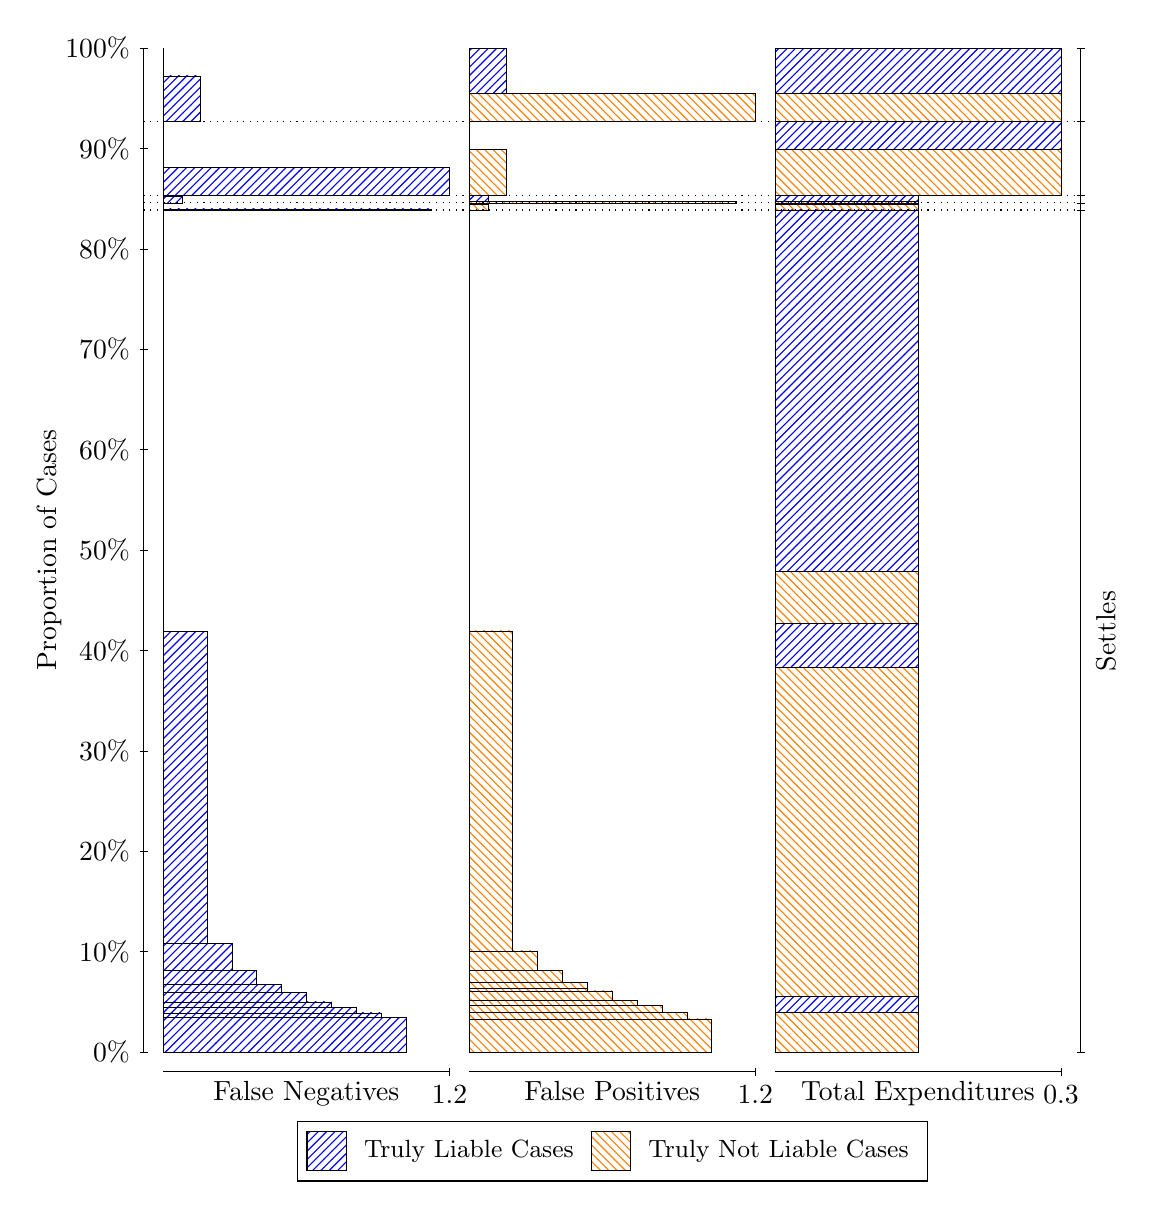
\begin{tikzpicture}
\draw[black, very thin] (1.5,1.75) -- (1.5,14.5);
\node[rotate=90, anchor=center] at (0.3, 8.125) {Proportion of Cases};
\draw[black, very thin] (1.45,1.75) -- (1.55,1.75);
\node[anchor=east] at (1.45, 1.75) {0\%};
\draw[black, very thin] (1.45,3.025) -- (1.55,3.025);
\node[anchor=east] at (1.45, 3.025) {10\%};
\draw[black, very thin] (1.45,4.3) -- (1.55,4.3);
\node[anchor=east] at (1.45, 4.3) {20\%};
\draw[black, very thin] (1.45,5.575) -- (1.55,5.575);
\node[anchor=east] at (1.45, 5.575) {30\%};
\draw[black, very thin] (1.45,6.85) -- (1.55,6.85);
\node[anchor=east] at (1.45, 6.85) {40\%};
\draw[black, very thin] (1.45,8.125) -- (1.55,8.125);
\node[anchor=east] at (1.45, 8.125) {50\%};
\draw[black, very thin] (1.45,9.4) -- (1.55,9.4);
\node[anchor=east] at (1.45, 9.4) {60\%};
\draw[black, very thin] (1.45,10.675) -- (1.55,10.675);
\node[anchor=east] at (1.45, 10.675) {70\%};
\draw[black, very thin] (1.45,11.95) -- (1.55,11.95);
\node[anchor=east] at (1.45, 11.95) {80\%};
\draw[black, very thin] (1.45,13.225) -- (1.55,13.225);
\node[anchor=east] at (1.45, 13.225) {90\%};
\draw[black, very thin] (1.45,14.5) -- (1.55,14.5);
\node[anchor=east] at (1.45, 14.5) {100\%};

\draw[black, very thin] (13.4,1.75) -- (13.4,14.5);
\draw[black, very thin] (13.35,1.75) -- (13.45,1.75);
\node[anchor=west] at (13.35, 1.75) {};
\draw[black, very thin] (13.35,12.443) -- (13.45,12.443);
\node[anchor=west] at (13.35, 12.443) {};
\draw[black, very thin] (13.35,12.534) -- (13.45,12.534);
\node[anchor=west] at (13.35, 12.534) {};
\draw[black, very thin] (13.35,12.629) -- (13.45,12.629);
\node[anchor=west] at (13.35, 12.629) {};
\draw[black, very thin] (13.35,13.566) -- (13.45,13.566);
\node[anchor=west] at (13.35, 13.566) {};
\draw[black, very thin] (13.35,14.5) -- (13.45,14.5);
\node[anchor=west] at (13.35, 14.5) {};

\draw[black, very thin, pattern color=blue, pattern=north east lines] (1.75,1.75) rectangle (4.8304,2.1882);
\draw[black, very thin, pattern color=blue, pattern=north east lines] (1.75,2.1882) rectangle (4.5145,2.2452);
\draw[black, very thin, pattern color=blue, pattern=north east lines] (1.75,2.2452) rectangle (4.1986,2.3204);
\draw[black, very thin, pattern color=blue, pattern=north east lines] (1.75,2.3204) rectangle (3.8826,2.3859);
\draw[black, very thin, pattern color=blue, pattern=north east lines] (1.75,2.3859) rectangle (3.5667,2.5043);
\draw[black, very thin, pattern color=blue, pattern=north east lines] (1.75,2.5043) rectangle (3.2507,2.6071);
\draw[black, very thin, pattern color=blue, pattern=north east lines] (1.75,2.6071) rectangle (2.9348,2.7822);
\draw[black, very thin, pattern color=blue, pattern=north east lines] (1.75,2.7822) rectangle (2.6188,3.1293);
\draw[black, very thin, pattern color=blue, pattern=north east lines] (1.75,3.1293) rectangle (2.3029,7.0961);
\draw[black, very thin, pattern color=orange, pattern=north west lines] (1.75,7.0961) rectangle (1.75,12.443);
\draw[black, very thin, pattern color=blue, pattern=north east lines] (1.75,12.443) rectangle (5.1464,12.458);
\draw[black, very thin, pattern color=orange, pattern=north west lines] (1.75,12.458) rectangle (1.75,12.534);
\draw[black, very thin, pattern color=blue, pattern=north east lines] (1.75,12.534) rectangle (1.987,12.614);
\draw[black, very thin, pattern color=orange, pattern=north west lines] (1.75,12.614) rectangle (1.75,12.629);
\draw[black, very thin, pattern color=blue, pattern=north east lines] (1.75,12.629) rectangle (5.3833,12.983);
\draw[black, very thin, pattern color=orange, pattern=north west lines] (1.75,12.983) rectangle (1.75,13.566);
\draw[black, very thin, pattern color=blue, pattern=north east lines] (1.75,13.566) rectangle (2.2239,14.147);
\draw[black, very thin, pattern color=orange, pattern=north west lines] (1.75,14.147) rectangle (1.75,14.5);
\draw[black, very thin, pattern color=orange, pattern=north west lines] (5.6333,1.75) rectangle (8.7138,2.1696);
\draw[black, very thin, pattern color=orange, pattern=north west lines] (5.6333,2.1696) rectangle (8.3978,2.2486);
\draw[black, very thin, pattern color=orange, pattern=north west lines] (5.6333,2.2486) rectangle (8.0819,2.3389);
\draw[black, very thin, pattern color=orange, pattern=north west lines] (5.6333,2.3389) rectangle (7.7659,2.4077);
\draw[black, very thin, pattern color=orange, pattern=north west lines] (5.6333,2.4077) rectangle (7.45,2.5261);
\draw[black, very thin, pattern color=orange, pattern=north west lines] (5.6333,2.5261) rectangle (7.1341,2.5589);
\draw[black, very thin, pattern color=orange, pattern=north west lines] (5.6333,2.5589) rectangle (7.1341,2.6345);
\draw[black, very thin, pattern color=orange, pattern=north west lines] (5.6333,2.6345) rectangle (6.8181,2.7874);
\draw[black, very thin, pattern color=orange, pattern=north west lines] (5.6333,2.7874) rectangle (6.5022,3.0328);
\draw[black, very thin, pattern color=orange, pattern=north west lines] (5.6333,3.0328) rectangle (6.1862,7.0965);
\draw[black, very thin, pattern color=blue, pattern=north east lines] (5.6333,7.0965) rectangle (5.6333,12.443);
\draw[black, very thin, pattern color=orange, pattern=north west lines] (5.6333,12.443) rectangle (5.8703,12.519);
\draw[black, very thin, pattern color=blue, pattern=north east lines] (5.6333,12.519) rectangle (5.6333,12.534);
\draw[black, very thin, pattern color=orange, pattern=north west lines] (5.6333,12.534) rectangle (9.0297,12.549);
\draw[black, very thin, pattern color=blue, pattern=north east lines] (5.6333,12.549) rectangle (5.8703,12.629);
\draw[black, very thin, pattern color=orange, pattern=north west lines] (5.6333,12.629) rectangle (6.1072,13.213);
\draw[black, very thin, pattern color=blue, pattern=north east lines] (5.6333,13.213) rectangle (5.6333,13.566);
\draw[black, very thin, pattern color=orange, pattern=north west lines] (5.6333,13.566) rectangle (9.2667,13.919);
\draw[black, very thin, pattern color=blue, pattern=north east lines] (5.6333,13.919) rectangle (6.1072,14.5);
\draw[black, very thin, pattern color=orange, pattern=north west lines] (9.5167,1.75) rectangle (11.333,2.2567);
\draw[black, very thin, pattern color=blue, pattern=north east lines] (9.5167,2.2567) rectangle (11.333,2.4544);
\draw[black, very thin, pattern color=orange, pattern=north west lines] (9.5167,2.4544) rectangle (11.333,6.6365);
\draw[black, very thin, pattern color=blue, pattern=north east lines] (9.5167,6.6365) rectangle (11.333,7.1931);
\draw[black, very thin, pattern color=orange, pattern=north west lines] (9.5167,7.1931) rectangle (11.333,7.8508);
\draw[black, very thin, pattern color=blue, pattern=north east lines] (9.5167,7.8508) rectangle (11.333,12.443);
\draw[black, very thin, pattern color=orange, pattern=north west lines] (9.5167,12.443) rectangle (11.333,12.519);
\draw[black, very thin, pattern color=blue, pattern=north east lines] (9.5167,12.519) rectangle (11.333,12.534);
\draw[black, very thin, pattern color=orange, pattern=north west lines] (9.5167,12.534) rectangle (11.333,12.549);
\draw[black, very thin, pattern color=blue, pattern=north east lines] (9.5167,12.549) rectangle (11.333,12.629);
\draw[black, very thin, pattern color=orange, pattern=north west lines] (9.5167,12.629) rectangle (13.15,13.213);
\draw[black, very thin, pattern color=blue, pattern=north east lines] (9.5167,13.213) rectangle (13.15,13.566);
\draw[black, very thin, pattern color=orange, pattern=north west lines] (9.5167,13.566) rectangle (13.15,13.919);
\draw[black, very thin, pattern color=blue, pattern=north east lines] (9.5167,13.919) rectangle (13.15,14.5);
\draw[black, dotted] (1.5,12.443) -- (13.4,12.443);
\draw[black, dotted] (1.5,12.534) -- (13.4,12.534);
\draw[black, dotted] (1.5,12.629) -- (13.4,12.629);
\draw[black, dotted] (1.5,13.566) -- (13.4,13.566);
\draw[black, very thin] (1.75,1.5) -- (5.3833,1.5);
\node[anchor=north] at (3.5667, 1.5) {False Negatives};
\draw[black, very thin] (5.3833,1.45) -- (5.3833,1.55);
\node[anchor=north] at (5.3833, 1.45) {1.2};

\draw[black, very thin] (5.6333,1.5) -- (9.2667,1.5);
\node[anchor=north] at (7.45, 1.5) {False Positives};
\draw[black, very thin] (9.2667,1.45) -- (9.2667,1.55);
\node[anchor=north] at (9.2667, 1.45) {1.2};

\draw[black, very thin] (9.5167,1.5) -- (13.15,1.5);
\node[anchor=north] at (11.333, 1.5) {Total Expenditures};
\draw[black, very thin] (13.15,1.45) -- (13.15,1.55);
\node[anchor=north] at (13.15, 1.45) {0.3};

\node[black, centered, rotate=90] at (13.72, 7.0963) {Settles};





\draw (7.449999999999999,1.5) node[draw=none] (baseCoordinate) {};
\begin{scope}[align=center]
        \matrix[scale=0.5, draw=black, below=0.5cm of baseCoordinate, nodes={draw}, column sep=0.1cm]{
            \node[rectangle, draw, minimum width=0.5cm, minimum height=0.5cm, pattern=north east lines, pattern color=blue] {}; &
            \node[draw=none, font=\small] (B) {Truly Liable Cases}; &
            \node[rectangle, draw, minimum width=0.5cm, minimum height=0.5cm, pattern=north west lines, pattern color=orange] {}; &
            \node[draw=none, font=\small] (B) {Truly Not Liable Cases}; \\
            };
\end{scope}

\end{tikzpicture}
\end{document}